% Chapter 7

\chapter{Evaluation and Improvements} % Main chapter title

\label{Evaluation and Improvements} % For referencing the chapter elsewhere, use \ref{Chapter1} 

\lhead{Chapter 7. \emph{Evaluation and Improvements}} % This is for the header on each page - perhaps a shortened title

%----------------------------------------------------------------------------------------


\section{Formative evaluation}
Formative evaluation is evaluation that takes place during the design process and is used to improve a design \citep[p. 149]{Hartson}. It focuses on identifying usability problems in a prototype that should and can be addressed during an iterative design process. It also ensures that users continue to be included in development - their feedback being central to improving the design \citep{GabbardHix}. 

The goal of the formative evaluation process was firstly to determine that the high-fidelity prototype was an accurate representation of the paper prototype, according to the users' conceptual models, and secondly to establish that the interface met the high-level user requirements determined earlier in the design process.

Following the process outlined by Gabbard et al.  \citep{GabbardHix}, user questions and tasks were developed to test all functionality and behaviour of the interface. In particular, the tasks were designed to test the user requirements and use cases that emerged from the requirements analysis process and the paper prototyping sessions, such as being able to filter annotations, search for particular annotations and view those made by specific users. The test was practised informally (with a willing family member) before users were involved, to ensure that the wording of questions and tasks made sense and that the evaluator was comfortable with the test material.

Users were first asked interview-type questions to assess their conceptual interpretation of the interface. Without interacting with the system (they could move the mouse and hover over elements, but not click on anything), users were asked what they thought various visual components represented, and how they would expect them to behave when they interacted with them. These questions were designed to determine initial user expectations and assumptions, and were phrased such as "\textit{what do you think xx represents?}" and "\textit{what would you expect to happen if you clicked on yy?}". 

Users were then asked to complete the tasks (with free use of the mouse or keyboard), which were contextualised with reality-based scenarios.


The test questions are documented as follows.

\textbf{To test interface components:}
\begin{enumerate}
 \item What do you think the left-hand area of the page represents?
 \item What do you think will happen if you interact with anything the left-hand side of the page?
  \item What do you think the rows in the table represent?
  \item What do you think each group of checkboxes represents? 
   \begin{enumerate}
    \item What do you think will happen if you click on an "All" checkbox?
    \item Do you think the greyed-out checkboxes are clickable? If so, what do you expect to happen if you clicked on one of them?
   \end{enumerate}
  \item What do you think the text box beneath the checkboxes is for?
  \item What do you expect will happen if you start typing into that box?
  \item What do you think the button labelled "Reset" does?
  \item What do you think the zoom cursor on mouseover means?
  \item Do you think the rows are clickable? If so, what do you think would happen if you clicked on a row?
  \item In the column called "Annotation information", what do the four bold pieces of text at the top of each cell refer to?
  \item What do you think the little arrows in the top row of the table mean?
  \item Do you think the table is sorted by default? If so, why do you think so? And how do you think it's sorted? 
\end{enumerate}

\textbf{To test interface behaviour:}
\begin{enumerate}
 \item Let's say you've been asked to find all annotations made in Physical Sciences. What would you click on?
 \item Without using your mouse, how many annotations do you think there there? How do you know this?
 \item Say you want to refine your search to all annotations in Physical Sciences, Grade 10. What would you click on?
 \item Next, what if you want to refine your search to all annotations in Physical Sciences, Grade 10, Chapter 5. What would you click on?
 \item Let's assume you've found the annotation you were looking for and now you'd like to clear your search and return to the initial view of the page. What would you click on or do to achieve this? (To reload the page/reset to defaults.)
 \item If you'd like to find all annotations that users have labelled as being comments. What would you click on?
 \item Let's say a user calls the office to ask if his annotation has been captured in the system. His username is "bob" (all lowercase). You need to find all the annotations by this user. What would you do first?
 \item If you need to find all annotations made by users with usernames starting with lowercase "s", what would you do?
 \item Let's say you're not sure about a user's comment and would like to view the original webpage where the webbook text was annotated. How would you go about this?
 \item What if you'd like to view all suggestion type annotations at the top of the table:  what would you do to sort them? 
 \item Let's say you need to find the annotation with the highest number of replies. What would you do to find this?
 \item You'd like to know more about the annotation with the highest number of replies. What would you do [if anything] to find more information about this annotation and its replies? 
 \begin{enumerate}
 \item  What text do you think was annotated by the original user? [Assuming user clicks on an annotation]
 \item Who do you think was the original user? Why do you think this?
 \item What do you think the original user's comment on the text was? Why do you think this?
 \item Which user do you think replied first to the original annotation, and when did they do it? Why do you think this?
 \item What do you think that user's reply was? Why do you think this?
 \item If you'd like to go back to the main page/view. what would you do?
 \end{enumerate}
 \item Let's say you need to check that there aren't any annotations in subjects other than Maths, Maths Lit or Physical Sciences (e.g. Biology). How would you go about this? What would you click on first?
 \item You've been asked to check that no annotations have mistakenly been made under Maths Lit Grade 11. How would you go about doing this? What would you click on first? 
 \end{enumerate}
 

\subsection{Usability test results}
\underline{User A} thought that the greyed-out sub-checkboxes did not look clickable. He also thought that the username search box looked greyed-out. He was uncertain as to how the username search box would behave: while he noticed there was no "Search" button to submit a user search he did not know if the search box would "\textit{filter on the fly}" or offer an auto-complete drop-down list of matching usernames. He said it was not always obvious that the table rows had actually updated once he had interacted with a filter.

He realised that the zoom icon (when hovering on a table row) indicated expansion, but was not sure what information an expanded view would include. He commented that the cursor did not change if he hovered over the table header sort icons, so it did not seem clear that the sort arrows were clickable because: "\textit{When you can click on things you get the finger}" (
\includegraphics[width=0.5cm]{Figures/handcursor.png}). He also noticed that when hovering over the table header text (e.g. "Type") the cursor changed to be a text input cursor (
\includegraphics[width=0.5cm]{Figures/textcursor.png}). This was a default DataTables/browser behaviour which the evaluator had not noticed in testing before.

In addition, User A noticed the DataTables CSS bug already mentioned, where in some instances the fixed table header cells do not align correctly with the table data cells in the rows beneath them.

To close the detailed view overlay, he tried clicking off the box, which did not work - he felt it "\textit{probably should}". He also mentioned that he thought the "Reset" button was "\textit{a bit obscured}" at the bottom of the page, and suggested renaming it to "Reset Filters" and moving it to the top of the page. 

\underline{User B} also did not think that the greyed-out sub-checkboxes were clickable - she assumed they would become clickable if she unchecked "All". She also expected the "All" checkbox to be an all/none toggle, so that if "All" was unchecked, then nothing would be selected. When she realised this was not the case (unchecking an "All" selected all the sub-checkboxes instead), she deselected the sub-checkboxes to get to the required filter set. For example, to select the "Chapter 5" filter - she unchecked the "All", which selected the 24 sub-checkboxes for "Chapter" and proceeded to deselect 23 checkboxes until just "5" was selected. Even though she realised this was inefficient and unlikely to be the only solution, she did not experiment with the checkbox behaviour to see if an alternative option was available. 

The purpose of the username search box was not initially clear to her as she did not know what it would be used to search for. She also was not sure how it would behave and whether she would have to press [Enter] to submit a search, for example. Once she interacted with the search box however, she realised that it filtered the table automatically. 

User B also missed the visual indication of the default date sort (
\includegraphics[width=0.4cm]{Figures/sortarrowdown.png}). She realised the table was sorted by date, but she deduced this from the date column entries.

\underline{User C} did assume that the greyed-out sub-checkboxes were clickable. However, when she interacted with the system, she first tried to deselect one, and then discovered that clicking on one actually selected it. However, she did not think to deselect all subject checkboxes to get no results in the table. 

She did not expect anything to happen if she started typing in the username search box, and she mistook the "Reset" button for a username "Search" (submit) button: she assumed she would have to type in the box and then press "Reset" to submit her user search. 

When she started interacting with the interface it was apparent that her confusion about the "Reset" button extended beyond this: after she selected the relevant group of checkboxes to a particular task she clicked the "Reset" button to submit her entire filter query (i.e. she did not notice the table updating at all) and then was perplexed when she realised her filter choice had just been cleared. According to her: "\textit{I would want to choose something and then click something else.  It would make sense if you had some instructions. I think it's important to have a Reset button because there's quite a lot of options… But my initial thing is that you choose and click Enter [to] search. That's how you do it on Google}". 

User C thought that the zoom icon on row mouseover meant that the rows were clickable, but was not sure what clicking on a row would do ("\textit{either it would bring up more information, or single out that particular comment but I don't know how...}"). Eventually we established that she expected the zoom icon to indicate a literal, visual zooming in, i.e. making the text bigger ("\textit{why would you want to see it bigger, when you can read it?}"). She did not think that clicking on a row would bring up more detailed information and she only noticed that the URL in each row was clickable. 

She was uncertain as to how the "Annotation Information" column would sort itself, and was not sure why one would want to sort the table by "Type", when "\textit{you can do that with the filters on the left}". When she initially clicked on a sort icon, the table update was not obvious (the sorting change to the visible results was minimal), and this confused her. However she persevered and clicked again, and then realised that the table had updated. 

She thought that the coloured type labels looked like clickable buttons. She also noticed a bug where, even when there were no entries in the table, the counter text at the bottom still displayed "Showing 1 of 1 entries".

\underline{User D} did not think that the greyed-out sub-checkboxes were clickable in their initial state but thought they probably would be if the "All" checkbox was deselected (i.e. an all/some toggle). That being said, initially she did not try to click on a greyed-out sub-checkbox - she deselected "All" first and then clicked on a (already checked) sub-checkbox. She realised that this deselected the sub-checkbox. She experimented and discovered by accident that she could just select one greyed-out sub-checkbox directly. (For the chapter selection task where she discovered this alternative behaviour she said: "\textit{I wasn't going to uncheck them} [23 chapter numbers] \textit{all!}"). Interestingly, even after she realised she could just directly select a greyed-out sub-checkbox, for the next tasks she went to uncheck "All" again, first. Like User C, she did not think to deselect all subjects to get no results in the table. 

User D thought that the username search box was for "\textit{your username}" (i.e. that one would input your own username into the box, and that it was not a search). She did not expect typing into it to have any effect on the table. Then, in one task, she typed the text "Comment" in the box, to search for it. Based on this experiment, she then realised that the search box was specific, not general (i.e. not a site search), and then understood that it was to search for usernames in the table. In a later task, when she searched for "s" in the username search box, the table updated so quickly that she initially did not notice the results had changed.

She did not know what the sorting arrows in the table header indicated, and did not notice the Date default sort icon. She did not think that it was possible to sort by a column header until she tried clicking on the "Replies" header. When asked to sort by the highest number of replies she said: "\textit{I'd try and click here somewhere… [clicked] "Oh and that's what it does!}". She also noticed that the date sort, which at first glance looked correct, was in fact not (caused by a bug in the code that converted a long timestamp into human-readable text). 

User D did also not believe that the zoom icon indicated that the row was clickable. For her, it was not obvious that she could click on a row, or that doing so would surface additional details about that row. 

\underline{User E} initially thought that deselecting an "All" checkbox would result in one of the sub-checkboxes being selected. She did not think that the greyed-out sub-checkboxes were clickable, but said that the changing mouseover icon suggested that they were. She expected to have to uncheck the "All" checkbox first. When she actually interacted with the interface however, she tried clicking directly on a greyed-out sub-checkbox (without deselecting the "All") and realised that was possible. Despite this, she said "\textit{my instinct is still to uncheck 'All' first and then click on the others}".

With respect to the username search box, User E said that she hoped the table would not update until she had finish typing a username into the search box, because she was concerned that it would be very slow. She thought the search box might offer a drop-down list of auto-complete options, and said that that "\textit{would be good}". She initially assumed that she would need to hit [Enter] to submit her search, but then noticed that there was no "Search" button, so she assumed the search box must filter the table automatically. In a later task when she actually interacted with the search box, she noticed that it updated automatically as she typed. 

Like User A, User E said that she expected the cursor to change when she moused over the sort icons in the table header. She noticed that a three way sort was not possible and that she could not sort to have the "Errata" type at the top of the table. "\textit{It only has two...Then again I could just click on Errata} [in the type filter on the left] \textit{if I just wanted them}". She suggested the text "asc" and "desc" instead of just the sorting arrows - she felt that the arrows alone were visually too subtle. She also was not sure how the "Annotation Information" column would be sorted. 

For the detailed view overlay, like User A, she tried to click off the detailed view box to close it, which did not work. She also suggested using a "zoom out" icon when in the detailed view, to "\textit{match the zoom in icon}" which opened the detailed view in the first place. 

The above feedback can be summarised as follows:
\begin{itemize}
\item It was apparent that the behaviour of the checkboxes was not immediately obvious to users and that this needed to be re-evaluated. 
\item Additionally, the table often updated too quickly for users to notice that it had changed. 
\item The cursor icons on hover needed to be changed, to make it very clear where and when users could click on things (e.g. on the sort arrows but not on the header text). 
\item The sort arrows were not visually obvious enough.
\item The purpose of the "Reset" button was not immediately apparent, and users got confused as to whether or not it was related to the username search box. 
\item The purpose of the username search box was not clear enough, and users did not expect the automatic updating behaviour (of the table) associated with the search box. 
\item Users expected to be able to click off the detailed view to close the overlay. 
\end{itemize}
In addition, the evaluator also noticed a number of bugs and issues with the interface during the usability tests:
\begin{itemize}
\item A possible fix for the DataTables CSS \verb|<th>| bug needed to be investigated: at least one user noticed it and commented on the fact the the table header did not always line up.
 \item It was observed that clicking on the URL in a row triggered the OnClick event to open the detailed view. So, if a user clicked on the URL, the detailed view would open, and only then would the user be taken to the relevant Everything Maths/Science webpage. This needed to be fixed. 
\item It was also noticed that if a user had searched for a username, navigated away from the web page (e.g. to the Everything Maths/Science URL) and hit "Back" in the browser to return to the interface, the filters would all be reset on the page but the last string the user had searched for would still be visible in the username search box, which was misleading. 
\item It was noted that the numeric date sort did not work correctly because of the order in which the date components (year, month etc) were parsed by the JavaScript. 
\item It was also noted that not one user pressed the [Esc] key to exit the detailed view. 
\end{itemize}

Aside from these detailed issues, it was evident from the formative usability tests that the interface definitely provided users with news ways of interacting with a collection of existing annotations and made it possible to complete specific tasks realting to searching, sorting and filtering content. Users could view all information associated with an annotation, and view the webbook context in which the annotation was made. Users could filter by meaningful categories (such as subject and grade) and search for annotations made by a specific external user, and all in one interface (not across multiple, complicated views of the content).


\section{Improvements to the prototype}
Based on the above observations, improvements to the prototype were implemented as is detailed in the following sections. Due to the very small sample size, no meaningful statistical analysis could be performed on the test data \citep[p. 149]{Hartson}. Instead all user feedback was taken into consideration and where feedback was conflicting, changes were implemented according to best design practices (such as those detailed in Chapter 5), or the most universal design pattern possible.
\subsection{Checkbox behaviour}
A number of possible improvements were considered for the checkbox behaviour that was so clearly confusing users. Because another round of summative usability tests had already been planned, it was decided to make the smallest set of changes possible to the checkbox behaviour and then test those, instead of redesigning their entire functionality and behaviour. The logic was quite simply that the difficulties users had with the checkboxes could possibly be fixed with slight improvements and it was therefore worth pursuing a minimalist approach instead of redesigning larger components,  because any changes made could still be tested thoroughly.

The greyed-out checkboxes caused the most confusion because users did not think they could click directly on one of the sub-checkboxes when viewing the default state of the interface. The initial checkbox state was therefore changed so that no checkboxes were greyed-out, and only the "All" checkboxes were ticked (not the sub-checkboxes too).  

Additionally, sub-checkboxes were indented slightly, to make it more apparent that they were nested under each "All" checkbox (see Figure \ref{fig:newcheckbox}).

\begin{figure}[h!]
    \centering
    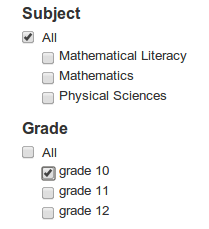
\includegraphics[width=0.4\textwidth]{Figures/V2/checkboxes.png}
 \caption{Improved checkboxes: no checkboxes were greyed-out and sub-checkboxes were indented.}
 \label{fig:newcheckbox}
\end{figure}


As from before, selecting a sub-checkbox would deselect the "All" checkbox associated with it. 

To perform an inverted selection (i.e. to select all sub-checkboxes, in order to deselect only a few) users could simply uncheck the "All" checkbox, which selects all the sub-checkboxes (see Figure \ref{fig:deselectedcheck}).

\begin{figure}[h!]
    \centering
    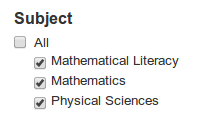
\includegraphics[width=0.4\textwidth]{Figures/V2/deselectAll.png}
 \caption{Deselecting an "All" checkbox selects all sub-checkboxes.}
 \label{fig:deselectedcheck}
\end{figure}


\subsection{Table reload speed}
The table reload speed was too fast, particularly when users were searching for a username and did not notice the table updating while their attention was focused on the username search box. 

While it would have been possible to slow down the reload speed slightly so that users would be more likely to notice the table updating \citep[p. 282]{Shneiderman1984}, this is not extensible or scalable behaviour: as soon as the table loads more than a certain number (unknown at this point) of annotations, its load time will become longer. It seemed impractical to deliberately introduce a slower table load speed, when the load speed will decrease anyway as the database grows, and at some point will become too slow and unresponsive (in which case server-side processing would be a better option). 

Whilst instantaneous responsiveness is desirable \citep[p. 272]{DixFinlay} and tolerable computer response times are well documented \citep[p. 154]{Nah} it would be more practical to make changes based on this with a system that is less of a prototype and more of an accurate representation of a real-world scenario (e.g. with thousands of annotations saved from multiple books), particularly because response time over the World Wide Web is so closely coupled to where the data processing occurs (client or server side). 

To alleviate confusion about the username search box automatically updating the table too quickly, a "Search" button was added to this filter (see section \ref{sec:searchbox}). 

\subsection{Cursors}
To clarify when users could click on elements, and what that clicking would result in, several hover cursors were changed to better conform to standard cursor patterns and usage:
The text cursor (
\includegraphics[width=0.5cm]{Figures/textcursor.png}) that appeared on hover over the table header text was removed (because the text is not editable)
The clickable 'finger' cursor (
\includegraphics[width=0.5cm]{Figures/handcursor.png}) was added on hover above the sort icons (in each table header cell) to indicate that they are clickable
In the detailed view overlay, a "Zoom out" cursor (
\includegraphics[width=0.7cm]{Figures/V2/zoomout.png}) was added on hover outside of the overlay, to mirror the zoom in icon and to indicate that clicking off the overlay would close it. 

\subsection{Sort icons}
The sort icons were made slightly larger and darker, to make them more visually obvious. In addition, the background colour for the table header row was changed, to improve contrast \citep[p. 650]{Galitz} of the sort icons on the background colour. 
\begin{figure}[h!]
    \centering
    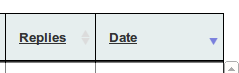
\includegraphics[width=0.4\textwidth]{Figures/V2/oldsort.png}
 \caption{Former sort icons and table header colour.}
\end{figure}

\begin{figure}[h!]
    \centering
    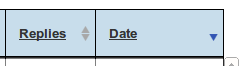
\includegraphics[width=0.4\textwidth]{Figures/V2/newsort.png}
 \caption{New sort icons and table header colour.}
\end{figure}

\subsection{Reset button}
The "Reset" button was renamed to "Reset Filters", to give users more information \citep[p. 520]{Galitz} as to its purpose. In addition, the styling between the username search box and the button was improved, to make it more apparent that the "Reset" button was not related to the username search box in functionality. 
\begin{figure}[h!]
    \centering
    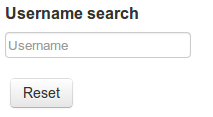
\includegraphics[width=0.4\textwidth]{Figures/V2/oldreset.png}
 \caption{The former "Reset" button.}
\end{figure}

\begin{figure}[h!]
    \centering
    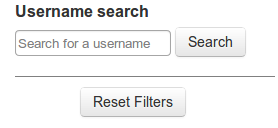
\includegraphics[width=0.5\textwidth]{Figures/V2/newreset.png}
 \caption{The new "Reset" button with improved microcopy and styling.}
 \label{fig:newreset}
\end{figure}


\subsection{Username search box}
\label{sec:searchbox}
To make it more clear to users what the purpose of the username search box was, the placeholder help text was changed from "Username" to "Search for a username". Additionally, a "Search" button was added, and the auto-updating of the table on search was removed so that users had to type text into the search box and then click the "Search" button (or press the [Enter] key) to submit their search. 

Whilst some users realised that the lack of a "Search" or "Submit" button probably meant that typing into the search box would update the table automatically, and noticed this behaviour when they used the filter, a number of users did not expect the search box to behave this way. Although the auto-updating was consistent with the behaviour of the other filters, it was decided to break that pattern and rather implement a "Search" button to cater for the latter group of users. The reasoning was that adding a "Search" button would cater for users who did not anticipate the automatic search, without alienating the users who appreciated the auto-updating, because the search box/"Submit" button is such a universal, familiar pattern (whilst being less directly consistent with other interface behaviour this is still supported by familiarity and generalisability design principles \citep[p. 264]{DixFinlay}). 

The search box outline was also made slightly darker, to avoid users thinking it was greyed-out.

\begin{figure}[h!]
    \centering
    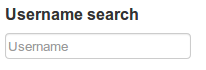
\includegraphics[width=0.4\textwidth]{Figures/V2/usernameold.png}
 \caption{The previous username search box.}
\end{figure}

\begin{figure}[h!]
    \centering
    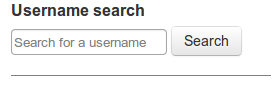
\includegraphics[width=0.5\textwidth]{Figures/V2/usernamenew.png}
 \caption{The new username search box with a search button and improved copy and styling.}
\end{figure}


\subsection{Closing the detailed view overlay}
Because a number of users tried to click off the detailed view overlay to close it, this functionality was added. 

\subsection{Bug fixes}
In addition to the improvements made to the interface as detailed above, fixes for the bugs discovered were also addressed. 

\subsubsection{DataTables CSS bug}
After thorough investigation, it was determined that the CSS table header bug introduced by DataTables' fixed header and vertical scrolling was not possible to fix. Because this is a minor styling issue that was only noticed by one user, it was left as is. In future it would be preferable to build customised tables with the necessary functionality instead of using the DataTables plugin, which would circumvent this bug.

\subsubsection{Table row onclick bug}
The OnClick behaviour of the table rows was tweaked, so that clicking on the URL in an "Annotation Information" cell did not open the detailed view overlay first, before going to the external URL. In addition, the external URLs were set to open in a new tab, so that users could open the page without inadvertently losing their current filter settings. 

\subsubsection{Username search caching issue}
To fix the bug that resulted in the last username search string displaying in the username search box if a user had navigated away from and back to the interface, the username search box text was modified to clear every time the page is loaded. 

\subsubsection{Date conversion/sorting}
The bug that resulted in the numeric date sort not working correctly was fixed. Quite simply the long UTC timestamp needed to be converted to a yyyy/mm/dd format (instead of dd/mm/yyyy) for the sort to work correctly. 

\subsection{Discussion}
The result of the above implemented changes was an interface that looked much the same as the original, but had subtle behavioural and stylistic differences (see Figure \ref{fig:newinterface}). 
\begin{sidewaysfigure}
    \centering
    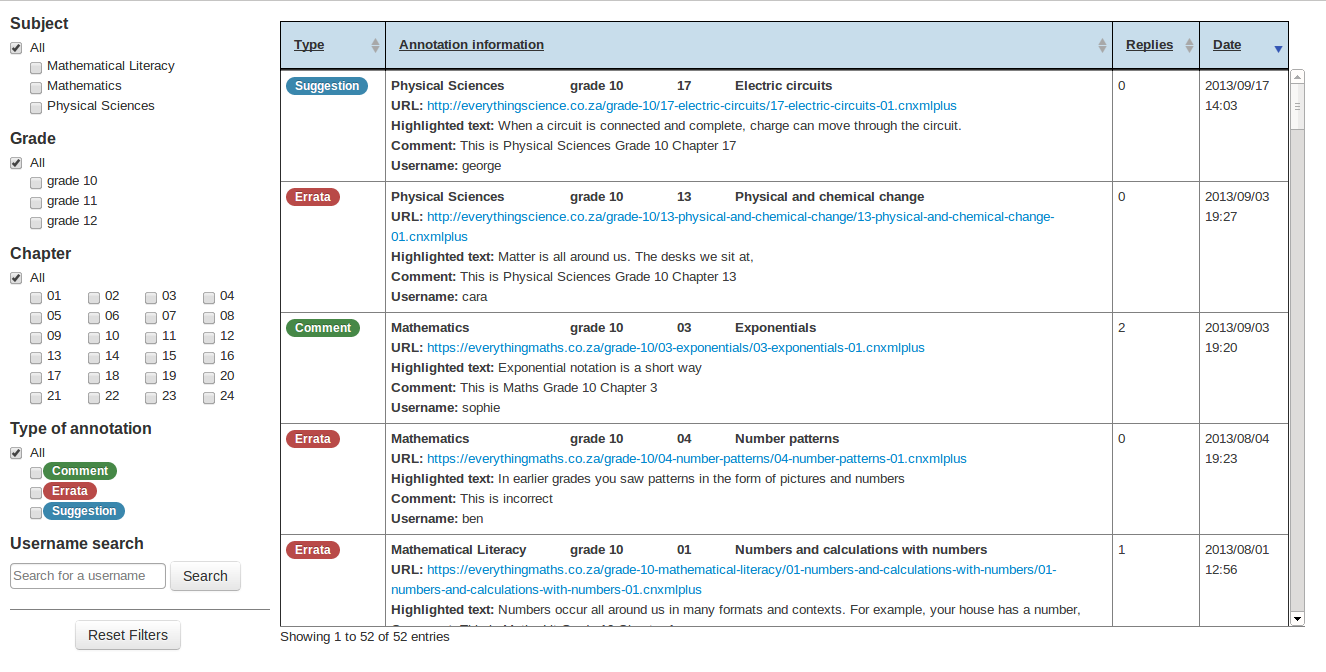
\includegraphics[width=\textwidth]{Figures/V2/wholeUI.png}
 \caption{The new username search box, with a "Search" button and better styling.}
 \label{fig:newinterface}
\end{sidewaysfigure}

With respect to the high-level goals of the interface, although many of the improvements made were subtle, they all fed into making the interface more intuitive and robust and aligning it more closely with the design guidelines and principles outlined in Chapter 4. Changes to behaviour (such as the checkboxes) made the interface more predictable and increased affordance \citep[p. 29]{RogersPreece}. Enhancing visual styles (such as the sort icon and table header colours, and the username search/reset button styling) made it easier for users to differentiate interface components, and therefore to determine their purpose. Fixing bugs such as the date conversion error corrected the layout of annotations and therefore improved consistency and predictability of the system. Improving the user experience in this way would make it easier for users to achieve their goals (including filtering, sorting, viewing and searching for annotations) without getting confused or distracted by unexpected behaviours from the interface. 


\section{Summative evaluation}
Summative evaluation is performed at the end of the design process, to "assess the success of a finished product" \citep[p. 437]{RogersPreece}. Whilst it is often comparative (i.e. comparing the performance of two interfaces \citep[p. 54]{GabbardHix}) in this case there was no alternative, existing interface with which to do a meaningful comparison. Additionally, whilst summative evaluation often includes statistical analysis \cite[p. 149]{Hartson}, the pool of available users who could be included in user tests was simply too small: a sample of 5 individuals is arguably not sufficiently large to perform meaningful quantitative analysis. 

Therefore, a qualitative summative evaluation process was undertaken, including usability tests, questionnaires and a heuristic evaluation. The goal of the evaluation was to assess whether or not the prototype did enable users to complete tasks including sorting, filtering and searching for annotations in an existing database.

For the summative usability tests five (new) users were selected, who again comprised a representative sample of the three user groups identified who would use the final interface ("Development", "Production" and "Sales").

Users were asked the same interview-style questions and to complete the same tasks as in the formative tests. This meant that results could be compared between the two sets of tests to confirm that the changes made were in fact improvements and better conformed to user requirements.

In addition, users were also asked to fill out several sections of the "Questionnaire for User Interaction Satisfaction" version 7 (QUIS7), to assess their satisfaction levels with the prototype interface \citep{QUIS}. 

As the final part of the summative evaluation, a heuristic evaluation of the interface was undertaken once usability testing was complete. 

\subsection{Usability test results}

\underline{User F} noticed that the interface has no overall "Submit" button and so assumed that the table would update itself automatically. He also noticed that it did in fact do so when he interacted with the system. In spite of this, between the first and second tasks, he clicked on "Reset Filters" to refresh the page, even though he did not need to do so. In the second task he realised that it was unnecessary to reset between filter interactions. 

He assumed that unchecking an "All" checkbox would produce in a "none" result (not "some") and was surprised when unchecking an "All" checkbox selected all the sub-checkboxes for that group (I.e. it inverted the selection). That being said he stated "\textit{I don't know why you would want a 'none' selection}". He did expect the indented sub-checkboxes to be directly clickable.

User F expected an auto-complete behaviour for the username search box. He noticed that the table did not update automatically when typing in the search box, and pressed the [Enter] key to submit his search. He also wondered whether it was possible to use wildcards when searching for a username.

With respect to the zoom icon on row mouseover he initially said that "\textit{when you zoom maybe it'll only show that comment. Visual zoom doesn't make sense because it's only text}". When he interacted with the interface however, he did not think to click on a row to view a single annotation.  When he was prompted by the evaluator to try clicking on a row he said "\textit{I'm not sure that's what zoom means}" (he clarified that he was in fact expecting a visual zoom, like Ctrl +) and "\textit{it sort of does what I expected...after I used it for the first time I'd know exactly what it does}". Once he had opened the detailed view, he used both the [x] button and clicking off the overlay to close it. 

User F did not notice the table column sort arrows initially, and was not immediately sure whether it was a descending or ascending sort. He also did not see the counter line of text (e.g. "Showing 1 of 26") at the bottom of table. He knew that sorting by type could be done using the sort arrows (though he realised a three way sort was not possible) or by using the left-hand "Type" filter. When using the sort arrows, clicking the first time did not produce the expected result (the column sorts by ascending results first so it does not always obviously change) and he hesitated before trying to click a second time (which did achieve the correct sort for that task).

He noticed that the number of chapters in the filters on the left did not change depending on the subject and grade selection. He said he would have expected this and asked the (valid) question (when selecting Chapter 24 only, for all subjects):  "\textit{are there no comments} [annotations] \textit{for grade 11 and 12 because there are no chapters 24} [in those books] \textit{or because there are no comments?}"

He suggested replacing the long URLs in each annotation with hyperlinked text that described the book (Subject, Grade, Chapter) instead, and also suggested calling the URL a "Webpage" in case users did not know what a URL was. In addition, he suggested putting user comments (in the detailed view particularly) in quotes, to differentiate them from the other text.  

\underline{User G} assumed that a selected "All" checkbox meant that all the sub-check options were selected too and said that they should perhaps be checked too, when "All" was checked.  She expected unchecking "All" to mean "none" and was surprised when unchecking an "All" instead selected the sub-checkboxes for that filter. In the first task, she looked for a "Submit" button (to submit her filter selections) but then quickly realised that the table updated automatically. For one of the tasks it was not immediately apparent that the table had updated. She had noticed the counter text at the bottom of the table, so she scrolled down to see if that had changed (which it had - this confirmed for her that the table had updated). 

Like User F, she thought that the username search might offer an auto-complete or auto-prompt list of suggested usernames as she started typing. The first time she performed a username search she clicked on the "Search" button, and the second time she pressed the [Enter] key. 

She assumed that the zoom icon would "\textit{make it bigger in some way or maybe show just that row}" and simply clicked on a row to expand it when asked to find more information about an annotation. To close the detailed view she noticed the [x] button, but clicked off it when asked to perform the task. 

She also did not notice the default sorting arrow in the date column. She correctly thought that the table was sorted by date because she looked at the chronological timestamps. It was only once she had done this that she saw that the date column had a different sort arrow. To sort by 'suggestion' type, she used the left-hand filter instead of the sort arrows in the table. 

\underline{User H} thought that the checkboxes would be clickable (but not the text labels next to them). When she performed the first task (finding all Physical Sciences annotations) she clicked on the correct checkbox and then moved the mouse to hover over the username "Search" button. Although she did not click on it, it seemed as if she had not noticed the table updating automatically, and expected to have to submit her query. Later in the test, she said that the "\textit{table updates so quick you sometimes don't notice it}" and that she would prefer to select all the necessary filters and then click a "Submit" button, or to have a slower table update speed with a progress indicator, to make the table updating more obvious. She said she wanted the interface to "\textit{let me know that I've saved it} [the query]\textit{, let me know that I've submitted} [the query]". When asked to clear the table and find no annotations, she did not think to try deselecting an "All" checkbox and there was no indication that she expected an all/none toggle behaviour.

Like users F and G, she also expected the username search to offer some auto-complete functionality. She used the "Search" button and pressed the [Enter] key to perform her searches. 

User H thought that the zoom icon and row colour change on mouseover indicated that the row was clickable, and also thought that clicking would expand something somehow, but said she was not sure what to expect. When it came to the task requiring her to find more information about an annotation, she experimented and clicked on a row. Once in the detailed view, she knew she could click on the [x] button to close it, but instead clicked off the overlay. 

She noticed the sort icons in the table header, but did not notice the different default sort icon in the date column. She knew that the table was sorted by date (by default) but noticed this in the timestamps themselves and also said she would simply expect the information to be sorted by date with the latest annotations listed first. Like User F, when asked to perform a sort on the table, and the first click on a sort icon produced an ascending sort (instead of descending), she was momentarily confused and hesitated. A quick experimental second click on the sort icon completed the task however, and for the second sorting task she simply clicked twice, having learnt the behaviour of the sort. 

She noticed the counter line of text at the bottom of the table. She also did not assume that clicking on an annotation's URL would open it in a new tab - she deliberately right-clicked on the URL and selected the "Open in new tab" option. In one task, she got confused between the "Highlighted text" in an annotation and the "User comment", suggesting that it is possibly not obvious enough what the "Highlighted text" label means. 

\underline{User I} initially did not notice that the table updated automatically. In the first task she clicked on the correct checkbox, and clicked on the "Search" button next to the username search box. She repeated this pattern in the second task (find all annotations in Physical Sciences, Grade 10), despite saying "\textit{I wouldn't find 'Search' intuitive for all the filters - it looks like it's only for the username box.}" It was only when she performed the third task (find all annotations in Physical Sciences, Grade 10, Chapter 5) and the table changed dramatically that she realised she did not need to click the "Search" button.  

User I initially did not think that the username search box was for usernames only: she thought it could be a general search ("\textit{Say you had a vague memory of what you were looking for, you could search for a keyword or something from the title...}"). Like the other users, she also expected that the username search box would offer some kind of "\textit{suggestions}" in the way of auto-complete functionality. When using the searchbox, she clicked the "Search" button both times, and did not use the [Enter] key. Although she used the search box successfully to search for several usernames, when asked to see if there were any annotations in "Biology" she typed "biology" into the search box, whilst saying "\textit{it says username search so that would be problematic, but I would try 'biology' anyway.}" She did not think to deselect all of the visible subject options to see if that left any remaining annotations. 

While she noticed the sort icons in the table header, she (like the other users) did not notice the different default sort icon in the date column. She also did not notice that the timestamps were ordered. She said she just assumed the table might be ordered by date, by default, but she was not sure. To sort by 'suggestion' type, she did not try and use the filter on the left. Rather, she clicked on the sort icon twice, again - with a hesitation between clicks when the first click did not produce the desired result. She also noticed that it is only a two way sort, and that it therefore would not be possible to surface "Errata" at the top of the column ("\textit{I'm not sure why it's ordered in that way - where does errata go?}").

She noticed the counter line at the bottom of the table but said, interestingly "\textit{It says showing 1 of 26 annotations but I can see 5 of them in the table. So I would expect it to say '5 of 26' because there are 5 visible, not just 1}". 

To close the detailed view she noticed the zoom out icon and the [x] button but clicked off  the overlay to close it. 

\underline{User J} also expected that unchecking an "All" checkbox would mean a "none" was selected, which he said would be a "\textit{silly use case}". He said he expected a partial [-] indicator for an "All" checkbox when one of its sub-checkboxes was selected. He thought that the text labels (and coloured labels for type) next to the checkboxes might be clickable, and tried this. He soon realised the text itself was not clickable and so clicked on the checkbox itself. He also noticed  that there was "\textit{no button called 'Filter'}" and said that he expected to not have to submit his selection, i.e. that the table would update itself, and that the username search box might use live filtering as one typed. 

He assumed that the zoom in icon and row colour change meant that the row was clickable, and that more information was available, but was not sure exactly what to expect. One he opened the detailed view (by clicking on a row) he knew he could click on the [x] button to close it, but instead clicked off the overlay. 

He expected the up/down sort arrows to be two separate buttons. When asked to sort, he clicked on one half of the icon and then realised it was one button, and that the initial sort was performed the wrong way. He clicked again to get the correct sorting order. He was not sure how the "Annotation Information" column would sort but assumed (correctly) that the sort would start with the first row of information (subject, grade, and chapter number). He noticed the default sort triangle for the date column and  the ordered timestamps. 

When he used the username search box, he realised that it did not offer an auto-complete drop-down list of suggestions, nor did the table update automatically. He pressed the "Enter" key to submit both searches, and did not click the "Search" button. Between the two username search tasks he said (correctly) "\textit{I would not expect to have to click on 'Reset Filters' at this point}".

He noticed the counter text at the bottom of the table, and also noticed the bug that results in an empty table (with one row that says "No results to display" being paired with the line "Showing 1 of 1 entries" at the bottom of the table). 

When asked to check if there were any annotations in subjects other than the three listed, he said "\textit{I have no way of selecting something not in the list}" (he correctly assumed that the table and filters are populated from existing annotations only). Instead of trying to achieve a 'none' result by unchecking an "All" checkbox, he checked the number of entries for "All" subjects (52) and then selected the Maths, Maths Literacy and Physical Sciences checkboxes. This filter also produced 52 results, so he surmised that because there was no difference in tallies, there were no extra annotations in other subjects.

The summative usability tests revealed that all users were in agreement that:
\begin{itemize}
 \item the left-hand area of the interface represented some kind of filtering or navigation.
\item interacting with the left-hand area would somehow influence the table on the right.
\item each row in the table represented a set of  details about an annotation (or 'comment') made.
\item the "zoom in" icon represented expansion, and indicated that more would become visible, but no one was initially exactly sure what it would do.
\item clicking on an annotation's URL would take you to another web page.
\item to close the detailed view they could click the [x] button or simply click off the overlay (even if they did not notice the zoom out icon). No one used the [Esc] key to close the overlay. 
\item the "Reset Filters" button reset the interface to the default view and settings.
\end{itemize}
In addition, all five users correctly understood how information in the detailed view was grouped together, i.e. which comments, usernames and timestamps belonged together. 

To summarise the results of the second round of usability tests:
\begin{itemize}
\item All users expected the username search box to offer some kind of auto-complete function such as a drop-down list of suggested (known) usernames
\item While the functionality of the checkboxes was clearer, the behaviour of the "All" checkbox was still unexpected: all users expected an all/none toggle. 
\item Whilst everyone knew that the zoom in icon implied somehow seeing more, no one was certain what to expect. Several users did not notice the zoom out icon when in the detailed view overlay.
\item The sort icons were still not visible enough. The single purple arrow in particular went unnoticed several times. \item Additionally, the two way (ascending/descending) sorting was not always sufficient - e.g. for the three Types. Users also did not know what to expect from the "Annotation Information" column sort.
\item The counter text at bottom of table was not always noticed (some missed it) and was not always deemed accurate (e.g. "\textit{I can only see 5 results}" and the bug where it says "Showing 1 of 1 entries" when there are no annotations displayed)
\item The automatic updating of the table was once again not completely obvious to users (particularly when the changes to the table were more subtle), possibly because it was sometimes just too fast. As a result some users expect to have to select a variety of filters and then click a "Submit" button. 
\end{itemize}

While there are evidently still small improvements that could be made to enhance the user experience of the interface, the usability tests revealed that users could perform the tasks they needed to, including sorting, filtering, browsing, searching for, and viewing details about annotations. They could also achieve these goals more easily than the users from the formative usability tests, and there were fewer misconceptions and misclicks in the second round of tests - suggesting that many of the improvements made the interface were successful. 


\subsection{QUIS7 questionnaire}
No statistical analysis was performed on the QUIS7 data because the sample size (5 users) was too small for meaningful statistical results (the authors of QUIS recommend an ideal sample of $>$ 20 users for statistical purposes \citep{QUISquant}). Instead, a qualitative analysis of users' questionnaires was undertaken. 

Excluding the background sections of QUIS7 (parts 1 and 2) users answered 68 questions each (making a total of 340 questions) in parts 3, 4, 5, 6 and 7. Of those 340 questions, 7 were accidentally left unanswered. In some instances, users differed in their selection of the 'not applicable' option (e.g. for some questions one user listed the item as being 'N/A' while others rated it). These differences can most likely be attributed to different interpretations of the question and what the questionnaire terminology was referring to (particularly because the questionnaire is very generic).

Overall users' responses in the questionnaire were very positive. The vast majority of ratings were 7, 8 or 9 towards the positive end of the scale.  User ratings indicated that they found the system satisfying, stimulating, easy to use, and flexible (most ratings for the latter were neutral or tending towards flexible). Characters on the screen were easy to read and highlighting and bolding was helpful. Screen layouts were helpful, although User I indicated that the amount of information that can be displayed on the screen was inadequate (she mentioned in the usability test that she would like to see more table rows simultaneously). They also indicated that the sequence of screens was clear and predictable. According to User F "\textit{I found the layout fairly straight forward and easy to use. After the first time using it I pretty much knew how to navigate around the web page.}"

All users indicated that the terminology and messaging used throughout the system was consistent and that instructions were clear. For Question 5.2 however, user answers varied widely. The question is "Terminology relates well to the work you are doing?"  with 'always' at 1 on the scale and 'never' at 9 on the scale. One user selected 1 ('always'), one user failed to give a rating for the question, and three other users selected 7, 8, and 8 (i.e. tending towards "never"). 

The latter three choices are however completely inconsistent with the subset of questions relating to terminology, in which all user ratings were positive and indicated that computer terminology was used appropriately and terminology on the screen was precise. 

Question 5.2 is the only question in QUIS7 where the favourable outcome is at 1 instead of 9. It is therefore possible that users did not read the question carefully enough and assumed that it followed the same pattern as all other questions, with a rating of 9 being the 'best'. Because one user did not answer the question however, and because the sample size is so small, the ratings for this question probably require further investigation. 

Most users indicated that the computer kept them informed about what it was doing, although one user selected 'never' (1) for Question 5.5. All users indicated that performing an operation leads to a predictable result and that the length of delay between operations was acceptable. 

User opinions differed on the helpfulness of error messages (Questions 5.6 - 5.6.2) and whether it was possible to control the amount of feedback (Question 5.5.3). For the former, three users selected the 'not applicable' option, while one rated error messages as being neither helpful nor unhelpful (5) and the other rated them as being very helpful (8). With regards to controlling the amount of feedback, two users selected 'not applicable' whilst the other three gave ratings of 8, 9 and 6, where 1 is 'impossible' and 9 is 'easy'.

In the comments for Part 5, User F stated: "\textit{I find the terminology clear and concise}" while User G wrote "[There was] \textit{only one unpredictable thing - when I unticked the "All" button for Subject, all the subjects got ticked, whereas I expected them to remain unticked}". User J wrote "\textit{Using both 'Search' and 'Filter' is probably unnecessary. Non-technical users might find 'Search' more intuitive. Bold text is usually used for headings, but sometimes for important info - e.g. first line in each table row contains filter dimensions}".

All users indicated that learning to operate the system was easy and fast. One user rated the "learning advanced features" item with a 5, i.e. neither difficult nor easy. The same user also marked the three questions (6.2.2, 6.3 and 6.3.1) related to discovering new features, remembering names and use of commands and remembering specific rules about entering commands as 'not applicable'. The other users all indicated that these items were easy. All users indicated that tasks can be performed in a straight-forward manner, that the number of  steps per task was just right and that the steps followed a logical sequence. 

User comments for Part 6 included "\textit{I find it really easy to learn to use the system", "Very easy to learn. [I] Feel safe exploring and actions are intuitive and rememberable. Only [a] 5 min learning curve}" and "\textit{There are apparently keyboard shortcuts but they were never displayed on the screen - so no opportunity to learn them}", which is true and should be corrected.

In terms of system capabilities (Part 7) all users indicated that the system speed, response time and rate at which information is displayed are fast enough. Similarly, they all rated the system as reliable and operations as dependable. Most users indicated that it was easy to correct mistakes and typos.  However one user selected the 'not applicable' option for these two questions. 

With respect to Question 7.5 ("ease of operation depends on your level of experience"), one user rated this item with a 1 ('never') whilst the other two users gave it a 7 (tending towards 'always'). Unfortunately the other two users failed to answer the question, so this result is ambiguous and again probably needs further investigation. 

All users indicated that one can easily accomplish tasks knowing only a few commands and that features and shortcuts can be used with relative ease (the lowest rating for this last question 7.5.2 was a 6).

User comments for Part 7 of the questionnaire included "\textit{It was pretty clear after using the system what capabilities it had and also its limitations}" and "\textit{it is easy to use} [the] \textit{interface without experience}".

In summary, whilst there were two questions that wielded slightly perplexing results, and some questions that only a subset of users marked as being 'not applicable', generally feedback gathered from the questionnaire was very positive. The results indicate that users generally found the system easy to learn and to use and that their overall reactions to the interface were favourable, which correlates to the findings from the usability tests.

\subsection{Heuristic evaluation}
As part of the summative evaluation, a heuristic evaluation of the interface was performed. Heuristic evaluations and usability tests have been shown to be supplementary evaluation methods which can be used to identify different kinds of usability problems \citep{Nielsen1995}. These two evaluation techniques along with standardised user feedback from the questionnaire therefore covered a fairly broad spectrum of evaluation when combined. 

The heuristic evaluation was performed by the designer/evaluator. It involved carefully progressing through tasks like those used for the usability tests, and evaluating each interface component and behaviour according to Nielsen's latest list of heuristics \citep{NielsenMack}. 

Whilst objectivity is undoubtedly hard to maintain when evaluating one's own work and it would have been preferable to have more than one evaluator participate in this process, time and resource constraints did not allow for this. Nonetheless, performing a heuristic evaluation resulted in a valuable higher-level analysis of the interface (as opposed to the very detailed results from the usability tests) according to standardised design guidelines.  It was an opportunity to gain some perspective by attempting to evaluate the interface within an established assessment framework, which is always a worthwhile undertaking.


The heuristic evaluation of the interface is as follows.
\begin{enumerate}
 \item \textbf{Visibility of system status}: Having the filters and corresponding (selected) annotations simultaneously visible in the interface provides users with as much information as possible. Because the checkbox selection directly affects the annotations displayed, a one-to-one mapping occurs, and the status of checkboxes on the left therefore serves as a kind of navigational indicator - what is ticked on the left corresponds to what a user can expect to see on the right. \\
 \\
 In some instances (particularly when changes to rows are minimal) it is arguable that the table updates too quickly for users to realise that it has changed - in this case appropriate visual feedback that the table has changed is too subtle, and made lead to confusion. \\ 
 \\
 Likewise, some of the sorts that can be performed on the table columns are too subtle. It is not always obvious to the user that anything in the table has changed.

\item \textbf{Match between system and the real world}: All filter labels (e.g. subject and type names, and words like "annotation", "username") come from stakeholder interviews and the paper prototyping sessions, and are commonly used in the users' workplace. Whilst the meaning of words for individuals might differ slightly, the microcopy and terminology used is appropriate to users who are familiar with technology, and the words and concepts used are sourced directly from their real world. Similarly, the filter hierarchy (subject > grade > chapter number) is duplicated in the real world in several workplace systems, including book authoring. Indeed, this structure is a common type of indexing and nesting in reality. 

\item \textbf{User control and freedom}: The system does not include any extended dialogues. The effects of a checkbox selection (or deselection) can be reversed by deselecting (or reselecting) the same box. The effects of a sort are reversible by simply clicking on the sort icons again. The detailed view overlay can easily be closed. Text in the username search box can easily be edited and searches can be resubmitted. If all else fails, a user can simply reset the entire interface to its default state using the "Reset Filters" button. The system therefore supports straightforward undo and redo in a number of instances.

\item \textbf{Consistency and standards}: The behaviour of the "All" checkbox is not consistent with conventions - these should be "all or nothing" toggles, not "all or something" toggles. The behaviour of other checkboxes is consistent with conventions however (and give the user an all or nothing selection). The behavioural inconsistency between the two kinds of checkbox is also not desirable and could be improved. \\
\\
The behaviours of scrollbars, the username search field and "Search" button, and the close ([x]) button in the detailed overlay are all standard. These elements behave as they would in any other software or system, and behave consistently within the system. \\
\\
The "zoom in" icon is not ideal. The icon is typically used to imply a literal visual zoom in other systems, whereas in this instance it implies something slightly different. That being said, no other standardised icon exists that would be more suitable. \\
\\
Between different parts of the interface, the same terminology is consistently used (e.g. the same labels are used for the same kinds of things across the system). 

\item \textbf{Error prevention}: No serious error-prone conditions exist in the system which is desirable. The "worst case scenario" a user can encounter is simply an empty table which displays the informative message that says "No results to display". \\
\\
Users cannot accidentally delete or lose data. Nonetheless it might be good to add a warning message that appears when users are about to navigate away from the page, to inform them that doing so will clear their current search, because the system does not handle any caching or use cookies. \\

\item \textbf{Recognition rather than recall}: Again, because all filter options are simultaneously visible on a single screen, users are not required to remember what selection they have made because it is visually apparent to them at all times. \\
\\
No instructions are included. Perhaps some help text on mouseover or simple instructions (e.g. "select a filter to update the table") would be beneficial. These should include keyboard shortcuts too (e.g. [F5] to refresh, or [Esc] to close overlay).

\item \textbf{Flexibility and efficiency of use}: The system is fairly simple and does not provide much in the way of options for novice or advanced users. That being said, it was designed for a very specific group of users who are all familiar with technology and use computers and web browsers on a daily basis.  Users cannot tailor frequent actions at present (e.g. save searches or set default filters). This would most likely depend on users being able to login before they start using the system, which would require server integration. 

\item \textbf{Aesthetic and minimalist design}: The design of the interface is minimalist: there are only two parts to the main interface, plus one overlay which is visually distinct (when the overlay is open, the rest of the page is is faded out). The microcopy used is generally concise and informative (e.g. the search placeholder text and filter labels). Less useful details (such as the in-depth info applicable to only one annotation) are hidden inside the detailed view and do not take up unnecessary space on the main page.  

\item \textbf{Help users recognize, diagnose, and recover from errors}: The system is generally error free (see error prevention discussion above). The error message given for an empty table is clear enough ("No results to display"). However it does not suggest a solution to remedy the situation. An extra line of help text to say "No results to display. Select a different filter", for example, would be an improvement. 

\item \textbf{Help and documentation}: The system does not include documentation. It is possibly simple enough that it does not need any. However, as mentioned already some inline help would be useful, for example to inform users about keyboard shortcuts. If the system were to be used by a completely different set of users (e.g. if the team were to expand, or the interface were to be used by a different company requiring similar functionality), more extensive documentation may well be necessary to acquaint them with the specific terminology and functionality used and designed for the users involved in this process.  
\end{enumerate}

To summarise possible improvements that emerged from the heuristic evaluation:
\begin{itemize}
 \item It is not always apparent that the table has updated itself after a filter selection. The same applies for some instances of column sorting. Some visual indication that the status of the system has changed would improve visibility of system status. 
 \item The behaviour of the "All" checkboxes is not consistent with checkbox behaviour in analogous systems. It is also not consistent with the behaviour of other checkboxes within this system. This should be amended to improve consistency.  
 \item The "zoom in" icon is potentially confusing: in other systems it suggests slightly different functionality. That being said, a more appropriate standardized icon is not available. 
 \item In terms of error prevention, adding a warning message that informs users that they will lose their current search if they navigate away from the web page would be helpful, to avoid this happening by mistake. 
 \item The empty table message could be more informative if it suggested how users can recover from this state, instead of just describing what has happened. Similarly, brief inline or mouseover help text (e.g. keyboard shortcuts) would be beneficial, to reduce the recall load on users and to provide useful, in situ documentation. 
 \item Including simple documentation about the system and how to use it would also be beneficial, particularly in the event that system is used by a different set of users to those for whom it was designed. 
\end{itemize}

The heuristic findings complemented much of the feedback from the usability tests and the QUIS7 results. Visibility of system status is good, as is the match between the system and the real world. There is much consistency with standard design patterns, the system is generally error free and the design is arguably aesthetic and minimalist. All of these factors suggest that the interface generally enables users to perform tasks, and does not hinder them. While the heuristic evaluation supports the notion that the interface does help users achieve new, high-level goals (e.g. sorting, filtering, searching, viewing annotation details) it also revealed the need for inline help text and possibly some simple documentation for the interface. 


\section{Discussion}
Overall the iterative, user-centred process of prototype design, formative evaluation, improvements to the design, and summative evaluation was a positive and constructive experience. It proved to be immensely useful to get user feedback in two stages and the feedback acquired from the formative design definitely helped to improve the design and iron out fundamental issues early on in development.

In terms of process, it would have been preferable to do testing with larger samples of users \citep{Faulkner}. This would have enabled meaningful quantitative data analysis (particularly of the QUIS7 data) which may have statistically aggregated and resolved differences between user opinions and experiences. Due to constraints within the company however, this simply was not possible. 

It is risky to attempt to aggregate information from such small samples \citep{Dicks} and any deviations (in behaviour, understanding or opinion) are significant and must be taken into consideration. With larger samples of users it would be easier to analyse the test results and attempt to determine trends in the data. Larger samples are also more likely to accurately represent an entire population (the "law of large number" principle in statistics), and can reduce issues associated with high variance \citep[p. 132 \& 235]{Gravetter}. 

It would also have been preferable to have more than one opinion on the heuristic evaluation \citep{NielsenHow}, and a more objective opinion at that. It is immensely difficult to remain neutral when analysing one's own work, particularly at the end of a lengthy development process. This is quite apart from the difficulties of having only one evaluator (no two evaluators consistently identify the same set of usability issues), as described by Hertzum and Jacobsen \citep{Hertzum}. 

Similarly, it would be irresponsible to ignore possible biases at play between users and the designer/evaluator \citep{Dumas}. Users who participated in the design process and testing are all colleagues of the designer, and it would be na\"{i}ve to assume that they could be completely objective about a project and interface designed for them, by an individual whom they know well. Similarly, as a designer so familiar with one's own company and team workflow processes, one must constantly guard against projecting assumptions, knowledge and workplace experience on to the design process.

Two other notes related to the summative evaluation include the importance of semantics and a possible pitfall in a heavily user-centred design process. 

Firstly, during usability tests the importance of the interpretation of words became apparent, with, for example, some users referring to a column sort as "filtering" (E.g. "\textit{I would filter by date}"). It is likely that the evaluator's understanding of some terminology is slightly different from various users' interpretations of the same terms. This could have affected answers to usability test questions, where it is possible that the evaluator's intention in a question was interpreted slightly differently by a user, due to subtle differences in the understanding of the language. 

Secondly, during the heuristic evaluation process, one thing that became evident was the lack of documentation. This occurred mainly because the system is designed for a small group of experienced, high-end users of technology who would likely not need extensive documentation to find their way around a relatively simple interface.  

Whilst following a user-centred process has undoubtedly resulted in an interface tailor-made to the said users' needs, it is interesting to consider how new users would experience the system, and whether or not it would be intuitive for them too. For example, if the company expands dramatically, would new employees also find the interface relatively straight-forward to use, or would they have (new) difficulties with it because it was not designed for them? All of this speaks to the extensibility of the system - how easily can it be reused or expanded. The possibility exists that a user-centred process with such a small group of users inadvertently resulted in a design that is not hugely extensible or remixable for a different set of users.

In summary, the formative evaluation revealed that the interface was largely successful at providing users with new functionality for interacting with annotations. Where the interface could be improved, it was, and the summative usability tests confirmed that many of the changes implemented did make the interface more intuitive and simple to use. While the usability tests, QUIS7 results and heuristic evaluation revealed that there are still small improvements that could be made, they also demonstrated that the interface was successful at providing users with the new functionality they required. In one interface, users were able to efficiently view, group, sort, filter and search for annotations - formerly tedious, if not impossible tasks. 

The final discussion about the success of the interface in terms of the original research question will be discussed in the following concluding chapter. 

